\documentclass[]{article}
\usepackage{graphics}
\begin{document}

\title{Quantum Computing and Grover's Algorithm}
\author{Matthew Hayward}
\maketitle
\pagebreak

\tableofcontents

\pagebreak

\section{Motivation for Study of Quantum Computing}

In the early 1980's physicist Richard Feynman observed that no
classical computer could simulate quantum mechanical systems without
incurring exponential slowdown.  [WC98] At the same time, it seems
reasonable that a computer which behaves in a manner consistent with
quantum mechanics could, in principle, simulate such systems without
exponential slowdown.  This possible violation of the Polynomial
Church-Turing thesis: ``any reasonable attempt to model mathematically
computer algorithms and their time performance is bound to end up with
a model of computation and associated time cost that is equivalent to
Turing machines within a polynomial.''  [EID00][Papadimitriou94]
Piqued much interest in the field.
	
At the same time, the evolution of classical computers has seen the
size of transistors and memory elements shrink exponentially.  These
components can not continue this trend indefinitely and still behave
in a classical manner.  At the current rate sometime around 2020 the
number of atoms used to represent a single bit of information will be
one.  [WC 98] At this scale the quantum behavior of the memory element
must be dealt with.

\subsection{A ``Killer App'' for Quantum Computing}

For many years the study of quantum computing was primarily an
academic curiosity, that changed rapidly in 1994, when Peter Shor
published his paper ``Algorithms for quantum computation: Discrete
logarithms and factoring.''  The primary result of the paper was a
polynomial time algorithm for factoring large integers.  [Shor94] It
is not known if there is a classical algorithm for factoring large
integers efficiently, but the best algorithms published thus far are
super-polynomial. [WC98] This algorithm coupled with the prominence of
cryptographic systems based on factoring large integers fueled study
of quantum computation, both from a algorithmic and a manufacturing
point of view.

Shortly after that, in 1996 L. K. Grover published his paper providing
a $O(\sqrt{n})$ time algorithm for finding a single marked element in
an unsorted database of $n$ elements.  [Grover96] The best possible
classical algorithm will run in $O(n)$ time.  This search problem was
not the first problem for which a quantum computer was shown to be
better than any possible classical computer, but it was the first
problem of real utility found where a quantum computer outperforms a
classical computer in an asymptotic sense. While Shor's algorithm may
be of more immediate utility, Grover's algorithm seems more
interesting in a theoretical sense, as it identifies substantial
efficiency for a real world problem in quantum computation.

\section{The Quantum Computer}

\subsection{The Qubit}

The bit is the fundamental unit of storage in a classical computer,
similarly, the basis of quantum computation is a qubit.  The qubit is
similar to a bit in that when measured its value will be either 0 or
1.  It differs primarily in what it is doing when it is not being
measured.  In particular, a qubit can exist in any superposition of
the 0 and 1 state simultaneously.  When a qubit in such a state is
measured the superposition will be destroyed.  It will be found to be
uniquely in the 0 or 1 state with some probability for each,
determined by the particulars of the superposition prior to the
measurement. [WC98]

\subsection{The Quantum Register}

A quantum register is just a group of qubits, all part of the same
quantum mechanical system.  Just as a $n$ bit register is capable of
representing $2^{n}$ distinct values, so too will a $n$ bit quantum
register assume one of $2^{n}$ basis states when measured. [WC98]

A quantum algorithm consists of a sequence of operations on that
register, to transform it into a state which, when measured, yields
the desired result with high probability.
	
Note that a $n$ bit quantum register can store an exponential amount
of information.  The register as a whole can be in an arbitrary
superposition of the $2^{n}$ base states which it can be measured to
be in.  While in this superposition, and computation applied to the
register will be applied to each component of the superposition, this
behavior follows from the linearity of operators on quantum mechanical
systems.  This behavior, called \emph{quantum parallelism} is the basis
for most quantum algorithms.

\subsection{A Formal Description of a Quantum Register}

The state of any quantum mechanical system is described by a state
vector in an appropriate Hilbert space.  A Hilbert space is a complex
linear vector space. [Greenwood00] This is similar to more familiar
vector spaces with the exception that vectors may have complex
lengths.  A linear vector space is one in which the sum or constant
multiple of a vector within the space is within the space as
well. [Griffiths95]

In the case of our $n$ bit quantum register, our Hilbert space will be
of dimension $2^{n}$.  The orthogonal basis for the Hilbert space can be
conveniently chosen to be the $2^{n}$ possible basis states that the
quantum register can be found in when measured.

With the chosen basis, the projection of the state vector on the i'th
basis vector will be the amplitude of the portion of the wave function
corresponding to the register being solely in the i'th state.

The state vector can be written $\Psi = (a_{1}, a_{2}, \ldots
a_{N})^{T}$, where $N = 2^{n}$.  $a_{i}$ is the amplitude of the wave
function in the i'th state, or equivalently the projection of the
state vector onto the i'th basis state.  The probability of measuring
the register in the i'th state is then: \[\frac{|a_{i}|^{2}}{\sum_{j = 1}^{N}|a_{j}|^{2}}\] where $|c|^{2} = c^{*}c$, here * is the
complex conjugate operator, so if $c = a+b\sqrt{-1}$, $|c|^{2} = a^{2}+ b^{2}$. [WC98] In general the amplitude of any component of the wave
function may be complex, but Grover's algorithm itself does not use
any complex amplitudes.

If we we insist that \[\sum_{j = 1}^{N} |a_{j}|^{2} = 1\] then the
probability of measuring the register to be in the i'th state becomes
simply $|a_{i}|^2$, where $a_{i}$ is the i'th component of the state
vector.  In this case we say the vector is normalized.

In the absence of measurement the state vector of any quantum system,
including our quantum register, will evolve according to the
Schr\"{o}dinger wave equation.  The Schr\"{o}dinger equation has the
property that if the solution is normalized at any time, it is
normalized at all times. [Griffiths95] Therefore if we initialize our
quantum register to be normalized, we can be sure that at all future
times the probability of measuring the quantum register in the i'th
state will be given simply by $|a_{i}|^{2}$.

A consequence of the Schr\"{o}dinger equation is that the evolution of
the system must be reversible.  At any point in time, if we know the
solution to Schr\"{o}dinger's equation, we can derive its solution at
all past and future times.  Thus any transformation we wish to perform
on our system should be reversible.  For our quantum register this
means that for any operation we use, we must be able to say what the
state of the register was before the operation, given the operation
and the resulting state. [Grover00] These remarks apply only to
quantum systems evolving in isolation of their environment.  Any
measurement of the register will irreversibly alter the system,
collapsing its wave function into one of its base states.

\section{Performing Computations}

Given the above constraints, it is not clear how to proceed in order
to have our quantum register undergo a transformation from an initial
state to some final state which performs a useful calculation.
Further, if we wish to make use of quantum parallelism, it is not
clear if the amplitude of the desired state will be large enough for
there to be a good chance of finding the register in this state.

Since an operation on our $n$ bit quantum register is simply a process
which transforms our state vector in our $N = 2^{n}$ dimensional
Hilbert space from state $\Psi = (a_{1}, a_{2}, \ldots a_{N})^{T}$ to
another state $\Psi^{'} = (a_{1}^{'}, a_{2}^{'}, \ldots
a_{N}^{'})^{T}$, we can represent any possible operator $\hat{T}$ as a
matrix:
	
	\[T = \left( \begin{array}{cccc}
	T_{11} & T_{12} & \ldots & T_{1N} \\
	T_{21} & T_{22} & \ldots & T_{2N} \\	
	\vdots & \vdots &        & \vdots \\
	T_{N1} & T_{N2} & \ldots & T_{NN} 
	\end{array}
	\right)
	\]

The matrix element $T_{ij}$ is the projection of the j'th component of
the input onto the i'th component of the output due to the
operator. [Griffiths95]

While mathematically any transformation can be achieved by assigning
the appropriate values to the matrix elements, only a very small class
of operators represent physically realizable operators on a quantum
system.  For a matrix to represent an operator which acts on a quantum
mechanical system, its effect on the state vector must agree with
conditions imposed by the Schr\"{o}dinger equation, namely the
operation must be reversible, and it must preserve normalization of
the state vector.

Physically realizable quantum transformations are reversible, thus we
are immediately restricted to consideration of operators whose matrix
representations are invertable, if the matrix representing the
operation $\hat{T}$ is singular (the determinant of $\hat{T}$'s matrix
representation is 0), it has no inverse, and thus can not be reversed.
So, invertability is a necessary, but not sufficient condition for a
matrix representation of a legal operator.

If we further require that the sum of the kinetic and potential energy
(called the Hamiltonian) of our system is not changing with time, then
the matrix representing any legal transformation will be ``unitary''.
A matrix $T$ is unitary if the transpose of the complex conjugate of
$T$ is $T^{-1}$.  [Griffiths95] So, we restrict our candidates for
operators to ones whose matrices are unitary, which will be a
necessary and sufficient condition for being a physically realizable
transformation on a quantum mechanical system with a time independent
Hamiltonian.  Systems with time dependent Hamiltonians' are also
feasible, but are not required to perform either Grover's or Shor's
algorithm, and are not considered here.

Now the specification of a quantum algorithm is simply a specification
for an initial normalized state vector of the quantum register, and a
series of unitary matrices representing legal transformations on that
state vector.  Eventually we will measure our register, and if our
operators are chosen well we will measure the register to be in a
desired state with high probability.

\section{Grover's Algorithm}

Assume you have a system with $N = 2^{n}$ states labeled $S_{1},S_{2},
\ldots S_{N}$.  These $2^{n}$ states are represented by $n$ bit
strings.  Assume there is a unique marked element $S_{m}$ that
satisfies a condition $C(S_{m}) = 1$, and for all other states $C(S) =
0$.  We assume that $C$ can be evaluated in unit time.  Our task is to
devise an algorithm which minimizes the number of evaluations of $C$.

The idea of Grover's algorithm is to place our register in a equal
superposition of all states, and then selectively invert the phase of
the marked state, and then perform an inversion about average
operation a number of times.  The selective inversion of the marked
state follows by the inversion about average steps have the effect of
increasing the amplitude of the marked state by $O(1/\sqrt{N})$.
Therefore after $O(\sqrt{N})$ operations the probability of measuring
the marked state approaches 1. [Grover96]

	Grover's algorithm is as follows: 
\begin{enumerate}
\item 
Prepare a quantum register to be normalized and uniquely in the first
state.  Then place the register in an equal superposition of all
states $\left(\frac{1}{\sqrt{N}},
\frac{1}{\sqrt{N}} \ldots \frac{1}{\sqrt{N}}\right)$ by applying the Walsh-Hadamard operator $\hat{W}$.  This means simply the state vector will be in an equal superposition of each state.

\item
Repeat $O(\sqrt{N})$ times the following two steps (the precise number
of iterations is important, and discussed below):

\begin{enumerate}
\item
Let the system be in any state $S$.  If $C(S) = 1$, rotate the phase
by $\pi$ radians, else leave system unaltered.  It is worth noting
that this operation has no classical analog.  We do not observe the
state of the quantum register, doing so would collapse the
superposition.  The selective phase rotation gate would be a quantum
mechanical operator which would rotate only the amplitude proportional
to the marked state within the superposition.

\item 
Apply the inversion about average operator $\hat{A}$, whose matrix
representation is: $A_{ij} = 2/N$ if $i \not = j$ and $A_{ii} = -1 + 2/N$ to the quantum register.
\end{enumerate}

\item
Measure the quantum register.  The measurement will yield the $n$ bit
label of the marked state $C(S_{M}) = 1$ with probability at least
$1/2$.

\end{enumerate}
[Grover96]

\subsection{An Illustration of Grover's Algorithm}

The following graphics illustrate the amplitudes of the varying states
of a 3 bit quantum register undergoing the steps to Grover's
algorithm:

Initially we prepare the register to be uniquely in the first state.

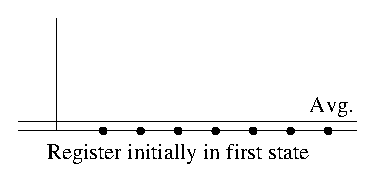
\includegraphics{init.eps}

We then perform the Walsh-Hadamard transformation on the register,
putting the register in a equal superposition of all 8 possible
states.

\includegraphics{wh.eps}

We then perform the selective phase inversion, which switches the sign
of the amplitude of the marked state, for the purposes of this
illustration the marked state is the fourth state.

\includegraphics{invert.eps}
	
Finally we perform the inversion about average operation, which
increases the amplitude of the state which was inverted in the
previous step.

\includegraphics{a.eps}


\subsection{Outline of Proof of Correctness of Grover's Algorithm}

To prove that Grover's algorithm successfully finds the unique marked
state in $O(\sqrt{N})$ operations we must show the following:

\begin{enumerate}
\item
That there is a operator to produce a equal superposition of states
for part 1 of the algorithm.  This operation is well known and referred
to as the Walsh-Hadamard operator.

\item 
That there is a operator to rotate the phase of a given state.

\item
That the definition of the matrix $A$ : $A_{ij} = 2/N$ if $i \not = j$
and $A_{ii} = -1 + 2/N$ is an inversion about average operator.

\item
That the matrix representations of all operators used are unitary.  If
this is the case then these transformations are physically realizable.

\item
That repeated applications of step 2 of the algorithm increase the
amplitude of the marked state, such that after $O(\sqrt{N})$
iterations the probability of measuring the marked state is at least
$1/2$.

\end{enumerate}

\subsection{Operator to Create Equal Superposition of States}

An equal superposition of states is created by the application of the
well known Walsh-Hadamard operator.  The matrix representing the
Walsh-Hadamard operator for an $n$ bit quantum register is a $2^{n}
\times 2^{n}$ matrix whose elements are defined to be: $W_{ij} =
2^{-n/2}(-1)^{\bar{i} \cdot \bar{j}}$, where $\bar{i}$ is the binary
representation of $i$, and $\bar{i} \cdot \bar{j}$ is the bitwise dot
product of the $n$ bit strings $i$ and $j$, $i$ and $j$ range from 0
to $(N-1)$, [Grover96] Put another way, $W_{ij} = \pm 2^{-n/2}$, where
the sign is positive if the bitwise AND of $i$ and $j$ has an even
number of 1's and negative otherwise. [Grover00]

The reason the Walsh-Hadamard operator inverts the sign (or rotates
the phase $\pi$ radians) in certain states is to allow it to be
reversible.  We are asking for an operator which places a quantum
system in an equal superposition of states.  For a classical
probabilistic system this would necessarily be a irreversible process,
as the resultant state would be the same for any input.  Since the
amplitudes of a quantum state can be complex, the probability of
measuring the a system in a given state is the absolute square of the
amplitude in the given state.  Thus the Walsh-Hadamard operation can
encode information in the phases of the states to make it reversible,
while still placing the register in a state where if measured any
basis state will be found with equal probability. [Grover00]

We may assume that prior to step 1 of our algorithm that our state is
prepared to be identically in one of the $N = 2^{n}$ basis states.
Assume that we place our register initially in the state where each of
the bits is zero, then the state vector for our $n$ bit register is:
$\Psi = (1, 0, 0, \ldots 0)^{T}$.  As a reminder, the state vector
$\Psi$ has $N = 2^{n}$ components, representing each of the states our
$n$ bit quantum register can be measured in.  After application of the
Walsh-Hadamard transformation the j'th element of the state vector is
$W_{0j} = 2^{n/2}(-1)^{\bar{0} \cdot \bar{j}}$, note that the bitwise
dot product of the zero vector and any $j$ vector is 0, thus the sign
of each amplitude is positive.

The result is an equal superposition of each state, all with positive
amplitude.  This was attained by performing the Walsh-Hadamard
operator to the register prepared solely in the first state.

Note that this can be done for a $n$ bit quantum register in $O(n) =
O(\lg N)$ time, although to simulate this on a classical computer we
must perform no less than $O(N)$ operations.  Here we see an example
of the kind of exponential slowdown in classical simulation of quantum
systems that Feynman observed.

\subsection{Operator to Rotate Phase}

The matrix representing an arbitrary rotation operator is very simple.
It takes the form of a diagonal matrix with $R_{ij} = 0$ if $ i \not =
j$, and $R_{ii} = e^{\sqrt{-1}\phi_{i}}$.  Here $\phi_{i}$ is an
arbitrary real number, and from Euler's formula we know the diagonal
entries may be equivalently written as $\cos{\phi_{i}} + \sqrt{-1}\sin{\phi_{i}}$. [Grover96]
	
For the selective phase rotation we will need such a matrix which
rotates only the phase of the marked state $\pi$ radians.  This will
be diagonal matrix with all ones on the diagonal, except the k'th
diagonal element will be -1 when the marked state is the k'th state.
Obviously we can not construct anything like this operator
classically, as to do so we would need to know the marked state in
advance.

How such a gate would be implemented in quantum mechanical system is a
little murky, I will leave it in Grover's own words: 

\begin{quote}
``In a practical implementation this would involve one portion of the
quantum system sensing the state and then deciding whether or not to
rotate the phase.  It would do it in a way so that no trace of the
state of the system be left after this operation (so as to ensure that
paths leading to the same final state were indistinguishable and could
interfere).  The implementation does \emph{not} involve a classical
measurement.'' [Grover96]
\end{quote}

We shall take the existence of such a gate as a given for the
remainder of the paper.

\subsection{Inversion About Average Operator}

We define the inversion about average operation on our state vector as
an operator that takes the amplitude of the i'th state, and increases
or decreases it so that it is as much above or below the average as it
was below or above the average before the operation. [Grover96]

The matrix representation of the inversion about average operator
$\hat{A}$ is defined: $A_{ij} = 2/N$ if $i \not = j$ and $A_{ii} = -1
+ 2/N$.  Note that $A = -I + 2P$ where $I$ is the identity matrix, and
$P$ is the matrix with each element is equal to $1/N$.  Observe that
$P$ has the following two properties, first $P^{2} = P$, and second
$Pv$, for any vector $v$, results in a vector $v^{'}$ with each
element being the arithmetic average of the the elements of
$v$. [Grover96]

Now we can examine the operation of $A$ on an arbitrary vector $v$.
$Av = (-I + 2P)v = -v + 2Pv$, By the second property of $P$ above,
note that $Pv$ is a vector with each element equal to $a$ where $a$ is
the arithmetic average of the elements of $v$.  Therefore the i'th
component of the vector is $(-v_{i} + 2a)$ which can be rewritten
$a+(a-v_{i})$.  Thus the i'th element is exactly as much above/below
average as it was below/above average before the operation. [Grover96]

\subsection{Proof that Operations are Unitary}

If the above matrices not unitary, they will not be physically
realizable, at least for systems with time independent Hamiltonians,
which are the only ones being considered here.  It must be shown that
each of the above operations is unitary.  As a reminder, a unitary
matrix is one whose inverse is the same as the transpose of its
complex conjugate, and unitary matrices represent reversible operators
that preserve normalization.

The Walsh-Hadamard transformation is one of the fundamental unitary
transformations used in quantum computing.  The proof is simply a
great deal of linear algebra, showing $W^{2} = I$ (since $W$ is real
and symmetric) and is omitted for brevity.

The rotation matrix $R$ with $R_{ij} = 0$ if $ i \not = j$, and
$R_{ii} = e^{\sqrt{-1}\phi_{i}}$.  Here $\phi_{i}$ is an arbitrary
real number.

It is easy to see $R$'s complex conjugate transposed is the inverse of
$R$.  When $R$ is multiplied by it's complex conjugate, the only
non-zero elements are on the diagonal, and when the diagonal elements
are multiplied the powers of $e$ will cancel, resulting in $e^{0} = 1$
on the diagonal, the identity matrix. [Grover96]

To show the inversion about average matrix $A$ is unitary, recall that
$A$ may be written as $A = -I + 2P$ where:
\begin{itemize}
\item $I$ is the identity matrix
\item $P$ is the matrix with each element is equal to $1/N$
\end{itemize}

Recall that $P^{2} = P$.  

$A$ is real and symmetric, so $A$ is its own transposed complex
conjugate, and we must show $A^{2} = I$.  

$A^{2} = (-I+2P)^2 = I^{2} - 2P - 2P + 4P^{2} = I - 4P + 4P = I$

[Grover96]

\subsection{Proof that Algorithm Increases Amplitude of Desired State}
	
Having established that the transformations in question are unitary,
and thus physically realizable, it is left to establish that
iterations of Grover's algorithm increase the amplitude of the marked
state $C(S_{m}) = 1$ enough that the probability of measuring state
$S_{m}$ is at least $1/2$ in $O(\sqrt{N})$ operations.
	
We start by examining the effect of the inversion about average
operator $A$.

\subsubsection{Theorem 1}

Theorem 1: Given the state vector of our register with one state with
amplitude $k$, and every other state with amplitude $l$, after an
application of $A$:
\begin{itemize}
\item the amplitude in the one state is $k^{'} = \left(\frac{2}{N} - 1 \right)k + 2\frac{(N-1)}{N}l$
\item the amplitude of the remaining $(N-1)$ states is $l^{'} = \frac{2}{N}k+\frac{(N-1)}{N}l$
\end{itemize}
	
Proof: Given the definition of $A$ as $A_{ij} = 2/N$ if $i \not = j$
and $A_{ii} = -1 + 2/N$, it follows from the definition of matrix
multiplication of $k$ and $l$ by $A$ that:
\begin{itemize}
\item $k^{'} = \left(\frac{2}{N} - 1 \right)k + 2\frac{(N-1)}{N}l$
\item $l^{'} = \frac{2-N}{N}l + \frac{2}{N}k + \frac{2(N-2)}{N}l$
\end{itemize} 
The second expression simplifies to $l^{'} = \frac{2}{N}k+\frac{(N-2)}{N}l$ with some simple algebraic
manipulation. [Grover96]

\subsubsection{Corollary 1.1}

Corollary 1.1: We seek to show that after applying $A$, both $k^{'}$
and $l^{'}$ are positive, under the following conditions:

Let the state vector for:
\begin{itemize}
\item one state have amplitude $k$
\item each of the remaining $(N-1)$ states the amplitude is $l$
\end{itemize}
And let:
\begin{itemize}
\item $k$ and $l$ be real
\item $k$ be negative, and $l$ be positive
\item $\left|\frac{k}{l}\right| < \sqrt{N}$
\item $N \ge 9$
\end{itemize}
Then, after applying $A$, both $k^{'}$ and $l^{'}$ are positive.

Proof: 

First we will show that $k^{'}$ is positive:
\begin{itemize}

\item From theorem 1 we know $k^{'} = \left(\frac{2}{N} - 1 \right)k + 2\frac{(N-1)}{N}l$.  

\item By assumption $k$ is negative. Since $N > 2$ by assumption, $\left(\frac{2}{N} - 1 \right)$ is negative.

\item By assumption $l$ is positive.  Since $N > 2$ by assumption, $2\frac{(N-1)}{N}$ is positive.

\item Thus the expression for $k^{'}$ is of the form $negative*negative + positive*positive$, which must be positive.
\end{itemize}

Next we will show that $l^{'}$ is positive:
\begin{itemize}
\item From theorem 1 we know $l^{'} = \frac{2}{N}k+\frac{(N-2)}{N}l$.

\item By assumption $\left|\frac{k}{l}\right| < \sqrt{N}$

\item For $N \ge 9$, $ \frac{(N-2)}{2} > \sqrt{N}$. Therefore when $N \ge 9$: $ \frac{(N-2)}{2} > \sqrt{N} > \left|\frac{k}{l}\right|$, and:

\[ l^{'} = \frac{2}{N}k+\frac{(N-2)}{N}l > \frac{2}{N}k + \left|\frac{k}{l}\right|l \]

\item Because $k$ is negative and $l$ is positive by assumption, $\left|\frac{k}{l}\right| = \frac{-k}{l}$.

\item Therefore: 

\[ l^{'} = \frac{2}{N}k+\frac{(N-2)}{N}l > \frac{2}{N}k + \frac{-k}{l}l = (\frac{2}{N}-1)k \]

\item It follows that $l^{'}$ is positive because $k$ is positive and
  $\frac{2}{N}-1 > 0$ for $N \ge 3$ (and by assumption $N \ge 9$).
\end{itemize}
[Grover96]

\subsubsection{Corollary 1.2}

Corollary 1.2: Let the state vector be as follows:
\begin{itemize}
\item For the marked state $S_{m}$ such that $C(S_{m}) = 1$, the amplitude is $k$
\item For all other $(N-1)$ states the amplitude is $l$
\end{itemize}
Then after the application of $A$:

\[ k^{2} + (N-1)l^{2} = k^{'2} + (N-1)l^{'2} \]

Proof: This follows directly from the fact that $A$ is unitary, and
that unitary transformations preserve normalization of the state
vector.  That means precisely that the sum of the absolute squares of
the components is the same before and after the operation.  Since we
never deal with any complex amplitudes in the processing of Grover's
algorithm, corollary 1.2 follows directly. [Grover96]

\subsubsection{Theorem 2}
	
Theorem 2: Let the state vector before step 2a of Grover's algorithm
be as follows:
\begin{itemize}
\item For the unique marked state $S_{m}$ which satisfies $C(S_{m}) = 1$ the amplitude is $k$ such that $0 < k < 1/\sqrt{2}$

\item For each of the remaining $(N-1)$ states the amplitude is $l$ such that $l > 0$
\end{itemize}
In this case we seek to prove both:
\begin{itemize}
\item The change in $k$, $\Delta k$ after steps 2a and 2b in Grover's algorithm is bounded below by $\Delta k > \frac{1}{2\sqrt{N}}$
\item After steps 2a and 2b in Grover's algorithm $l > 0$
\end{itemize}

Proof: Let the initial amplitudes be $k$ and $l$, let the amplitudes
after the selected phase inversion step 2a be $k^{'}$ and $l^{'}$, let
the amplitudes after the inversion about average step 2b be $k^{''}$
and $l^{''}$.
	
By theorem 1 we know $k^{''} = \left(1-\frac{2}{N} \right)k +
2\frac{(N-1)}{N}l$ (note the reversal of terms in the coefficient of
$k$, this is due to the phase inversion of $k$ in step 2a), therefore
$\Delta k = k^{''} - k = -\frac{2k}{N} + 2\left(1-\frac{1}{N}\right)l$.  
By the assumption $0 < k < 1/\sqrt{2} $ and Corollary 1.2 it follows
that $|l| > \frac{1}{\sqrt{2N}}$.  By assumption $l$ is positive, thus
$l > \frac{1}{\sqrt{2N}}$.  Combining this with $\Delta k = k^{''} - k
= -\frac{2k}{N} + 2\left(1-\frac{1}{N}\right)l$. it follows that
$\Delta k > \frac{1}{2\sqrt{N}}$. [Grover96]

To show $l^{''}$ positive consider after step 2a of the algorithm,
after the selective phase inversion, but before the inversion about
average. At this point $k^{'} < 0$ and $l^{'} > 0$, since $\left(0 < k
< \frac{1}{2\sqrt{N}} \right)$ and $|l| > \frac{1}{\sqrt{2N}}$ (from
previous paragraph) that $\left|\frac{k^{'}}{l^{'}}\right|< \sqrt{N}$.
This means that after step 2a our register is in a state covered by
Corollary 1.1, which states after the inversion about average
operation $l^{''}$ will be positive.


\subsection{A Special Case}

It is instructive to consider the special case of $N = 4$.  In this
special case, the precise number of iterations needed to attain the
correct measurement with unit certainty is one.  Thus it can provide
some intuition as to the manner in which Grover's algorithm exploits
interference between the states to raise the probability of the the
desired state. [Grover00]

In the case of $N = 4$ then, the entire Grover's algorithm is simply:
\begin{enumerate}
\item Qureg = $(1,0,0,0)^{T}$ (Quantum register in state 00 with probability 1)
\item Apply Walsh-Hadamard transformation to Qureg
\item if (C(Qureg) == 1) Apply Phase Inversion
\item Apply A transformation to Qureg (A is inversion about average)
\item Measure state of Qureg

Let us trace the evolution of our quantum register through the
algorithm.  Let us assume the state we are searching for is the state
three.  We will denote the state of our quantum register like this:
$(a,b,c,d)^{T}$, where the probability of measuring the register to be
in the state 00 is $a^{2}$, the probability of measuring state 01 is
$b^{2}$, the probability of measuring state 10 is $c^{2}$, and the
probability of measuring state 11 is $d^{2}$.  In general, the
amplitudes could be complex, but no complex amplitudes are used in
Grover's algorithm, so $a^{2} = |a|^{2}$.

For a 4 state system, the Walsh-Hadamard transformation is represented
by the matrix:
	\[W = \frac{1}{2}\left(\begin{array}{cccc}
	1 & 1 & 1 & 1 \\
	1 & -1 & 1 & -1 \\
	1 & 1 & -1 & -1 \\
	1 & -1 & -1 & 1 
	\end{array}\right)\]	

The inversion about average transformation is represented by the
matrix:
	\[A = \frac{1}{2}\left(\begin{array}{cccc}
	-1 & 1 & 1 & 1 \\
	1 & -1 & 1 & 1 \\
	1 & 1 & -1 & 1 \\
	1 & 1 & 1 & -1 
	\end{array}\right)\]	
\end{enumerate}

After step 1 of our algorithm the quantum register is in the state
$(1,0,0,0)^{T}$.\newline 
After step 2 of our algorithm the quantum register is in the state
$W*(1,0,0,0)^{T} = (.5,.5,.5,.5)^{T}$\newline
After step 3 of our algorithm the quantum register is in the state
$(.5,.5,-.5,.5)^{T}$.  Remember, the marked element in this example is
the third one.\newline
After step 4 of our algorithm the quantum register is in the state
$A*(.5,.5,-.5,.5)^{T} = (0,0,1,0)^{T}$.\newline
Now comes step 5, the measurement step, we can see that with unit
probability we will measure the state 3, which was the marked
state.\newline

Now, this is an exceptional case, in general we will not attain unit
probability after any number of iterations.  By theorem 2 we can see
that there is some number of iterations $m$ that is $O(\sqrt{N})$ such
that the probability of measuring the marked state is at least $1/2$.
Note that the result for monotonic increasing probability of the
marked state proved in theorem 2 only applies so long as the amplitude
of the marked state is less than $\frac{1}{\sqrt{2}}$.  Once the
amplitude is greater than that further applications of $A$ cause it to
shrink, it will then oscillate back and fourth as more applications of
the inner loop are executed. [BBHT96]

\section{Open Questions}

There are several open questions in Grover's paper.  Foremost among
these is how many times exactly should we iterate step 2 of Grover's
algorithm.  Grover proves the existence of some $m \in O(\sqrt{N})$,
such that after $m$ iterations of step 2 of the algorithm the
probability of finding the register in the marked state is greater
than $1/2$.  Since the amplitude of the desired state, and hence the
of probability of measuring the desired state, is not monotonic
increasing after $m$ iterations, it is not enough to know know the
existence of $m$, it's value must be determined.

\subsection{How Many Iterations are Required}

Our initial state $\Psi_{0} = (1/\sqrt{N}, 1/\sqrt{N}, \ldots,
1/\sqrt{N})$, is attained by performing the Walsh-Hadamard
transformation on the register in the zero state.

Let $(k,l)$ denote denote the state of our vector, where $k$ is the
amplitude of the marked state, and $l$ is the amplitude of each of the
remaining $(N-1)$ states.  It is the case in Grover's algorithm that
the unmarked states always have the same amplitude, so we can use this
shorthand.

After the first application of the Walsh-Hadamard operator to place us
in an equal superposition of states let us say we are in state
$\Psi_{0} = (k_{0}, l_{0})$.

From theorem 1 we see the j'th iteration will produce the state
$\Psi_{j} = (k_{j}, l_{j})$, where $k_{0} = l_{0} = 1/\sqrt{N}$,
further:

	\[k_{j+1} = \frac{N-2}{N}k_{j} + \frac{2(N-1)}{N}l_{j}\] 

	\[l_{j+1} = \frac{N-2}{N}l_{j} - \frac{2}{N}k_{j}\]

With a little work on the recurrence relation we an solve for closed
form solutions of $k$ and $j$.  Let the angle $\theta$ be defined so
that $\sin^{2}{\theta} = 1/N$.  It can be shown through mathematical
induction that:

	\[k_{j+1} = \sin{((2j+1)\theta)}\] 

	\[l_{j+1} = \frac{1}{\sqrt{N-1}}\cos((2j+1)\theta)\]
	[BBHT96]

We are interested in the number of iterations for $k$ to have near
unit probability.  Evidently, we will find the register to be in the
target state with unit probability when $(2m + 1)\theta = \pi/2$, or
when $m = (\pi-2\theta)/4\theta$.  We can only perform an integer
number of iterations, but the probability of failure is less than
$1/N$ if we iterate $\lfloor \pi / 4 \theta \rfloor$ times, which is
very close to $\frac{\pi}{4}\sqrt{N}$ when $N$ is large ($1/\sqrt{N} =
\sin{\theta} \approx \theta$).  [BBHT96] For the 50 percent
probability called for by Grover's algorithm we need only
$\frac{\pi}{8}\sqrt{N}$ iterations. [BBHT96]

\subsection{Searching for More Than One Item}

Grover briefly mentions that his algorithm can work in a setting where
there is more than one state such that $C(S_{i}) = 1$.  In fact this
poses no difficulty whatsoever, and regardless of the number of marked
states we retain our superior performance over classical algorithms..
If there are $t$ marked states, we can find one of the marked states
in $O(\sqrt{N/t})$ time.  This presumes that we know the number of
marked elements in advance. [BBHT96]

Another interesting special case comes when $t = N/4$, in this case
just as in the special case where $N = 4$, we will find a solution
with unit probability after only one iteration, which is twice as fast
as the expected running time for a classical algorithm, and
exponentially faster than the worst case classical running time.
[BBHT96]

\subsection{Optimality of Grover's Algorithm}

It is not directly proved, but simply stated in Grover's 1996 paper
that his result was optimal.

It was established in [BBBV96] that any quantum algorithm can not
identify a single marked element in fewer than $\Omega(\sqrt{N})$.
Grover's algorithm takes $O(\sqrt{n})$ iterations, and is thus
asymptotically optimal.

It has been shown since that any quantum algorithm would require at
least $\pi/4 \sqrt{N}$ queries, which is precisely the number queries
required by Grover's algorithm. [Grover99]

\subsection{Implications on P = NP}

A common fallacious argument made is that since any quantum algorithm
takes $\Omega(\sqrt{N})$ operations to identify a single marked
element in a database of $N$ elements, a quantum computer can not be
used to attain exponential speed up in a search problem.

This argument is incorrect because this lower bound applies only to
queries of the type used in Grover's algorithm, whose queries ask only
about a single database element at a time. [Grover97]

Various novel approaches can be used to get around the
$\Omega(\sqrt{N})$ queries barrier which still leave hope for a
finding some exponential speed up of an NP-Hard problem.  These
approaches generally try to capitalize on some structure of the
problem at hand, which Grover's algorithm does not do at all.

Grover provides an algorithm which will locate a single marked element
in a $N$ element database in exactly 1 query.  It does however require
$O(N\log{N})$ pre and post processing time. While much slower in
overall running time for the best classical and quantum algorithms for
the same task, it does demonstrate that the $\Omega(\sqrt{N})$ query
limit is not necessarily rule out exponential speed up of quantum
computers in a search problem.  [Grover97]

It has also been shown that nonlinear quantum mechanics imply
polynomial time solutions for NP-complete problems, however the same
paper notes that: ``Such nonlinearity is purely hypothetical: all
known experiments confirm the linearity of quantum mechanics to a high
degree of accuracy'' [Abrams98]

\section{Conclusion}

Quantum computation allows for exponential speed up and storage in a
quantum register via quantum parallelism.  The more basis states
represented within the register, and hence the more speed up due to
parallelism in the register, the more improbable it is that a desired
state can be measured.  Grover's algorithm handles this problem by
relying on transformations which cause the amplitude of the marked
state to increase at the expense of the non marked states, in a manner
ways this is analogous to interference of waves.

Grover's algorithm is unique among quantum algorithms in that it shows
a useful calculation that a quantum computer can calculate in fewer
operations than any classical computer possibly can. At the heart of
Grover's algorithm are two unitary transformations, the first is a
selective phase inversion, which makes the sign of the amplitude of
the target negative.  The second unitary transformation is an
inversion about average operation.  Initially we place the amplitude
of all states at the same positive value, each phase switch and
inversion about average increases the amplitude of the target state.
The exact number of times we perform these transformations is roughly
$\pi/4\sqrt{N}$ for sufficiently large $N$.  For a classical algorithm
the best time bound is $O(n)$.

\section{Bibliography}

	Items in the Los Alamos National Laboratory e-print quantum
	physics archives are available from
	\begin{verbatim}http://xxx.lanl.gov/archive/quant-ph\end{verbatim}

\begin{description}

\item{[Abrams98]}
D. Abrams, \emph{Nonlinear quantum mechanics implies polynomial-time
solution for NP-complete and P problems}, lanl e-print
quant-pt/9801041

\item{[BBBV96]}
C.H Bennett, E. Bernstein, G. Brassard and U. Vazirani, \emph{Strengths
and Weaknesses of Quantum Computing}, to be published in the SIAM
Journal of Computing.

\item{[BBHT96]}
M. Boyer, G. Brassard, P. Hoyer and A. Tapp, \emph{Tight Bounds on
Quantum Searching}, Proceedings, PhysComp 1996 (lanl e-print
quant-ph/9701001)

\item{[EID,00]}
Eppstein D., Irani S., and Dillencourt M. \emph{ICS 260-Fall,
2000-Class Notes 11: Turning Machines, Non-determinism, P and NP}
\begin{verbatim}http://www1.ics.uci.edu/~eppstein/260/notes/notes11.ps \end{verbatim}

\item{[Greenwood00]}
G. Greenwood, \emph{Finding Solutions to NP Problems: Philosophical
Differences Between Quantum and Evolutionary Search Algorithms} lanl
e-print quant-ph/0010021

\item{[Griffiths95]}
D. Griffiths, \emph{Introduction to Quantum Mechanics}, Prentice Hall,
Inc.  Upper Saddle River, NJ 07458

\item{[Grover96]}
L. Grover, \emph{A fast quantum mechanical algorithm for database
search}, Proceedings of the 28th Annual ACM Symposium on Theory of
Computing 1996, pp. 212-219

\item{[Grover97]}
L. Grover, \emph{Quantum computers can search arbitrarily large
databases by a single query}, lanl e-print quant-ph/9706005

\item{[Grover99]}
L. Grover, \emph{How fast can a quantum computer search?}, lanl
e-print quant-ph/9809029

\item{[Grover00]}
L. Grover, \emph{Searching with Quantum Computers}, lanl e-print
quant-ph/0011118

\item{[Papadimitriou94]} 
Papadimitriou, C. \emph{Computational Complexity} Addison-Wesley
Publishing Company, 1994

\item{[Shor94]}
P. Shor, \emph{Algorithms for quantum computation: Discrete logarithms
and factoring}, Proceedings of the 35th Annual IEEE Symposium on
Foundations of Computer Science 1994, pp. 124-134

\item{[WC98]}
C. Williams, S. Clearwater, \emph{Explorations in Quantum Computing},
Springer-Verlag, New York, Inc.

\end{description}

\end{document}
